Il rover utilizzato è un robot a quattro ruote ricavato da una macchina giocattolo RC, attuato da due motori: uno per lo sterzo mentre l'altro per la trazione. Di seguito vengono descritti i principali componenti e sensori utilizzati. la parte software del rover è controllata tramite il modulo Nvidia Jetson AGX orin.

\subsection{Nvidia Jetson AGX Orion}
Il kit per sviluppatori NVIDIA Jetson AGX Orin  \cite{Nvidia} e tutti i moduli Jetson Orin condividono un'unica architettura SoC, consentendo di emulare prestazioni e potenza per qualsiasi modulo. È configurato per impostazione predefinita per coloro che utilizzano i moduli della serie Jetson AGX Orin, ma può essere facilmente riprogrammato per emulare i moduli della serie Jetson Orin NX o Jetson Orin Nano. \\
La scheda carrier inclusa espone molte interfacce hardware standard, consentendo una piattaforma altamente flessibile ed estensibile per la prototipazione rapida.

\subsection{ZED}
La fotocamera ZED \cite{ZED} è progettata per replicare il funzionamento della visione umana. Utilizzando le due camere e la triangolazione, la ZED fornisce una comprensione tridimensionale della scena osservata.
Le caratteristiche principali sono:
\begin{itemize}
    \item Piattaforma di percezione spaziale end-to-end per capacità di rilevamento simili a quelle umane;
    \item Prestazioni in tempo reale, infatti tutti gli algoritmi dell'SDK ZED sono progettati e ottimizzati per funzionare in tempo reale;
    \item Ampia gamma di piattaforme supportate, dai PC desktop ai PC embedded.
\end{itemize}

\subsection{LiDAR}
L’acronimo LiDAR (Light Detection And Ranging) \cite{lidar} \cite{lidar2} identifica la tecnologia che  misura la distanza da un oggetto illuminandolo con una luce laser e che è  in grado di restituire informazioni tridimensionali ad alta risoluzione sull’ambiente circostante. Un LiDAR utilizza tipicamente diversi componenti: laser, fotorilevatori e circuiti integrati di lettura con capacità di tempo di volo per misurare la distanza illuminando un bersaglio e analizzando la luce riflessa.
Di base il LIDAR è una tecnica simile ad un radar basata sul principio dell‘eco.\\
L’utilizzo della tecnologia LiDAR comporta diversi vantaggi legati alla sua implementazione:
\begin{itemize}
\item Garantisce una misurazione veloce e precisa;
\item Ampia risoluzione: la luce ha lunghezze d’onda minori rispetto alle onde radio e questo aumenta la risoluzione del rilevamento e permette quindi di classificare meglio gli oggetti;
\item Semplicità e la facilità d’utilizzo.
\end{itemize}

\begin{figure} [H]
    \centering
    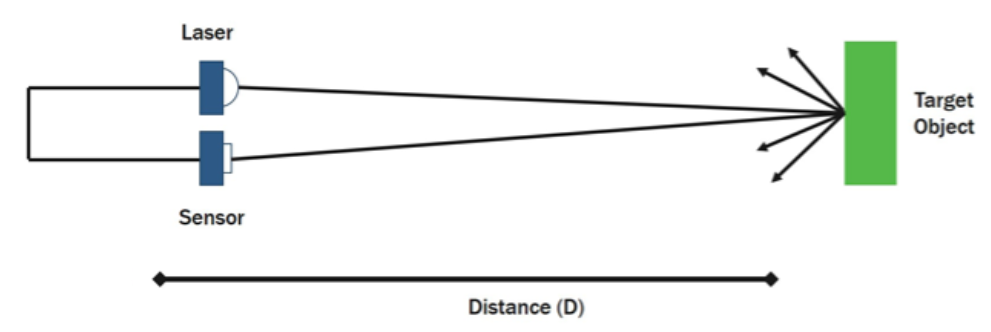
\includegraphics[width=0.5\linewidth]{img/Lidar.PNG}
    \caption{Funzionamento LiDAR}
    \label{fig:Lidar}
\end{figure}

In tale applicazione il LiDAR utilizzato è della marca YDLiDAR, modello G4, che ha le seguenti caratteristiche:
\begin{itemize}
\item Capacità di scansione a 360° (2D) entrambi i sensi di rotazione;
\item Offre una velocità di scansione di 9.000 scansioni al secondo con una portata di 16 m;
\item Comunicazione dati wireless.
\end{itemize}






